\chapter{Аналитический раздел}

\section{Постановка задачи}

В соответствии с заданием на курсовую работу необходимо разработать загружаемый модуль ядра для ОС Linux, осуществляющий контроль  проходящего через него сетевого трафика и позволяющий блокировать пакеты по заданному списку правил. Также необходимо предоставить пользователю возможность добавлять и удалять правила фильтрации пакетов, предусмотреть защиту от подмены ip-адресов, выводить информацию о DNS пакете, если обращение осуществляется по доменному имени.

Для достижения поставленной цели необходимо решить следующие задачи:
\begin{itemize}
	\item изучить принципы работы сетевой подсистемы Linux;
	
	\item проанализировать способы перехвата сетевых пакетов;
	
	\item ознакомиться со структурами и функциями ядра для работы с сетевыми пакетами;
	
	\item определить параметры, по которым будет осуществляться  фильтрация пакетов;
	
	\item реализовать межсетевой экран в виде загружаемого модуля ядра;
	
	\item протестировать работоспособность разработанного межсетевого экрана.
\end{itemize}

%\section{Процесс обмена информацией}

%OSI (Open Systems Interconnection) — концептуальная модель взаимодействия открытых систем, которая объединяет все коммуникационные функции вычислительных или телекоммуникационных систем. Эта модель состоит из 7 взаимозависимых слоев (уровней) ( таблица \ref{osi_table}), каждый из которых описывает путь данных от одной машины к другой и выполняет определенные функции  \cite{osi}.




\section{Принципы работы сетевой подсистемы Linux}
Сетевая подсистема Linux построена на стеке BSD. В этой подсистеме прием и передача данных на транспортном и сетевом уровнях модели OSI\footnote{OSI (Open Systems Interconnection) — концептуальная модель взаимодействия открытых систем, которая состоит из 7 взаимозависимых уровней, каждый из которых выполняет определенные функции~\cite{osi}} происходят с помощью интерфейса сокетов.

Когда в сетевую подсистему приходит пакет, возникает прерывание. Обработчик прерывания от сетевого адаптера копирует пакет в ядро, где тот ставится в так называемую буферную очередь и ожидает обработки соответствующим потоком ядра, и вызывает соответствующий softirq, который будет запущен демоном ksoftirqd и закончит обработку данного сетевого пакета (рисунок \ref{img:softirq})~\cite{ryaz}. 

Для обработки сетевых пакетов, поступающих с высокоскоростных интерфейсов, в Linux был добавлен NAPI (New API). В этом API механизм прерываний сочетается с механизмом опроса, и его основная цель -- сократить количество прерываний, генерируемых при получении пакета. В NAPI-совместимых драйверах при поступлении пакета прерывания отключаются, и обработчик только вызывает планировщик rx\_scheduler, который гарантирует, что в дальнейшем обработка пакета будет выполнена \cite{b5}.

%\clearpage
\begin{figure}[h]
	\centering
	\begin{center}
		{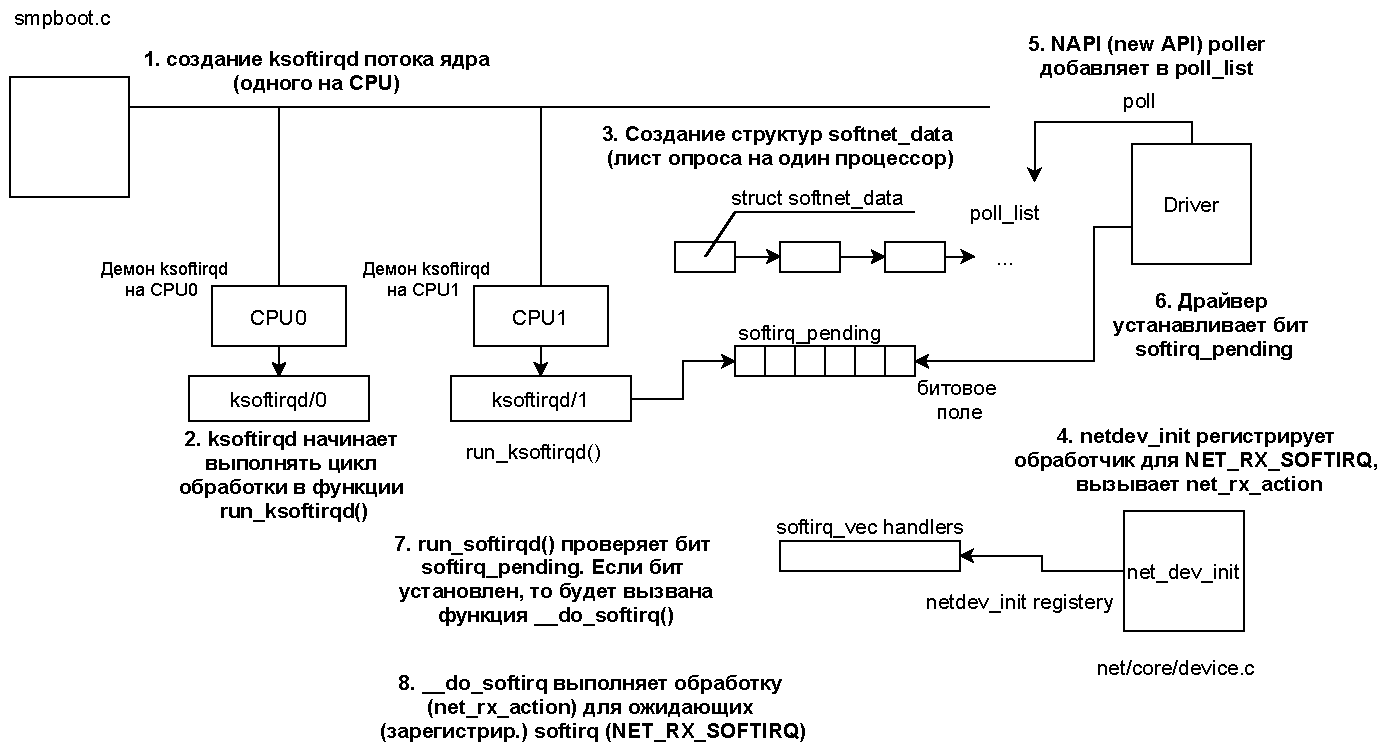
\includegraphics[scale=0.7]{inc/img/daemon.pdf}}
		\caption{Порядок выполняемых действий при приеме сетевого пакета}
		\label{img:softirq}
	\end{center}
\end{figure} 


%Сетевая карта записывает пакет в указанный адрес памяти, используя механизм прямого доступа к памяти (Direct Memory Access, DMA). Для этого в состав системы входит один или несколько контроллеров DMA, которые пересылают данные от внешнего устройства в оперативную память.



На рассматриваемых уровнях модели OSI и происходит фильтрация пакетов с учетом информации о протоколе и об IP-адресах и номерах портов источника и назначения. Широко распространённым средством фильтрации сетевых пакетов является библиотека Netfilter.

\section{Библиотека Netfilter}

Netfilter - это библиотека ядра Linux, предоставляющая функционал для фильтрации и перенаправления пакетов~\cite{b7}. Netfilter представляет собой набор перехватчиков внутри ядра, позволяющий модулям ядра регистрировать функции обратного вызова в сетевом стеке. Эти функции вызываются для каждого пакета, который удовлетворяет соответствующему правилу перехвата~\cite{netfilter}.


Netfilter позволяет перехватить пакет в любой из пяти стандартных точек, через которые он проходит (рисунок \ref{img:packets}):


\begin{enumerate}
	\item NF\_INET\_PRE\_ROUTING -- все входящие пакеты;
	\item NF\_INET\_LOCAL\_IN -- входящие пакеты, предназначенные для локального процесса;
	\item NF\_INET\_FORWARD -- транзитные пакеты (предназначенные для другого интерфейса);
	\item NF\_INET\_LOCAL\_OUT -- исходящие пакеты, сформированные локальными процессами;
	\item NF\_INET\_POST\_ROUTING -- все исходящие пакеты (поступившие из точки NF\_INET\_FORWARD или сформированные локальными процессами).
\end{enumerate}

\clearpage
\begin{figure}[h]
	\centering
	\begin{center}
		{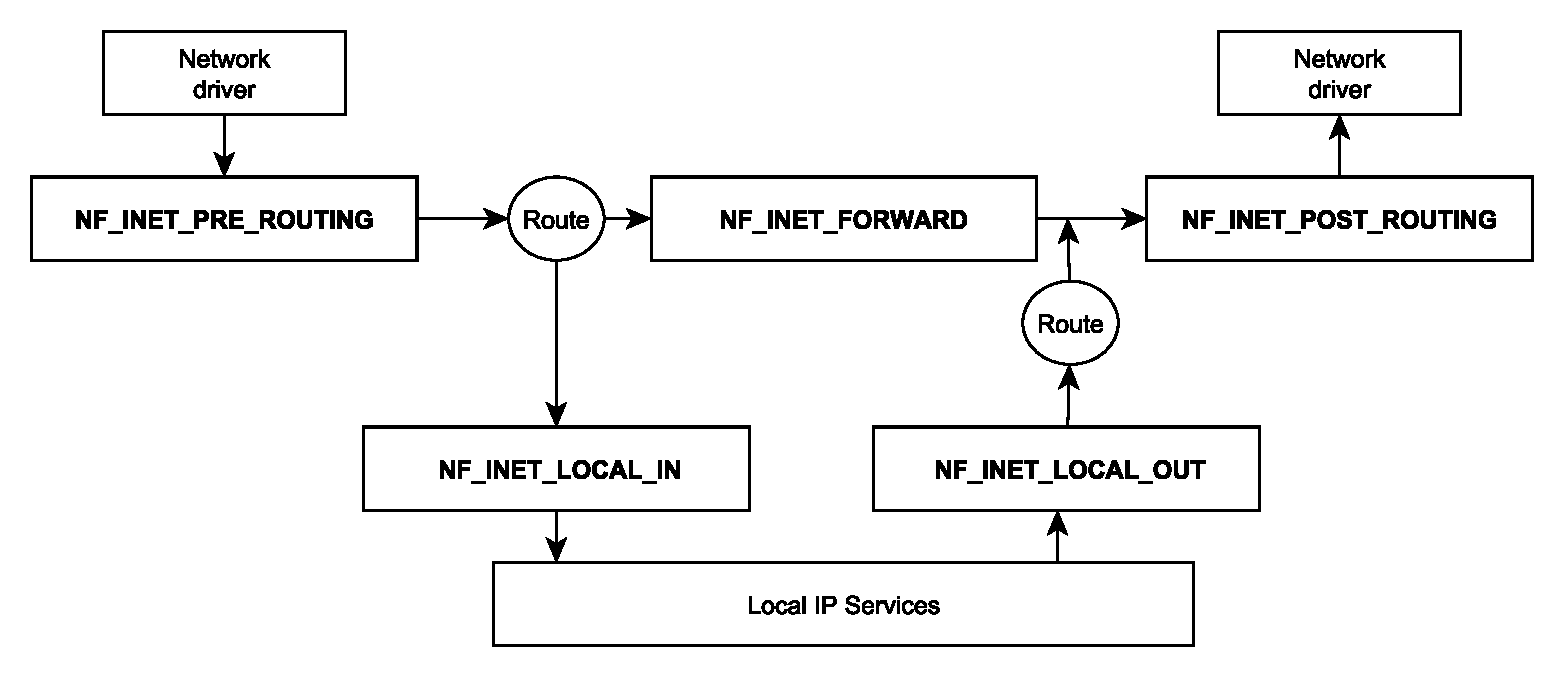
\includegraphics[scale=0.6]{inc/img/packets.pdf}}
		\caption{Точки, через которые проходит сетевой пакет}
		\label{img:packets}
	\end{center}
\end{figure} 


%Сетевые пакеты в Netfilter проходят последовательность цепочек (chain). Каждая цепочка содержит набор таблиц (table), которые представляют собой упорядоченные списки правил. Каждое правило содержит определенные параметры и указание на действие, которое необходимо выполнить при соответствии содержимого пакета параметрам~\cite{b7}.


\section{Функции перехвата}
Чтобы перехватить пакет в одной из перечисленных ранее точек, к ней необходимо подключить функцию перехвата (hook, ловушку). Для этого сначала необходимо заполнить структуру nf\_hook\_ops, основные поля которой приведены в листинге \ref{lst:hook}.

\begin{lstlisting}[caption = {Структура struct nf\_hook\_ops}, label=lst:hook]
struct nf_hook_ops {
	nf_hookfn		*hook;
	...
	u8			pf;
	...
	unsigned int		hooknum;
	int			priority;
};
\end{lstlisting}


Основные поля структуры:
\begin{itemize}
	\item hook -- функция, которая будет вызвана для обработки пакета и принятия решения: отбросить или принять пакет;
	
	\item pf -- семейство протоколов (PF\_INET для IPv4);
	
	\item hooknum -- точка подключения функции;
	
	\item priority -- приоритет (вводится, чтобы установить порядок вызова ловушек, подключенных к одной точке).
\end{itemize}

После заполнения структуры nf\_hook\_ops функцию перехвата необходимо зарегистрировать, вызвав функцию nf\_register\_net\_hook. Для удаления ловушки необходимо вызвать функцию nf\_unregister\_net\_hook. Прототипы этих функций приведены в листинге \ref{lst:hook_reg}.

\begin{lstlisting}[caption = {Функции для регистрации и удаления функций перехвата}, label=lst:hook_reg]
	int nf_register_net_hook(struct net *net, const struct nf_hook_ops *ops);

	void nf_unregister_net_hook(struct net *net, const struct nf_hook_ops *ops);
\end{lstlisting}



Прототип функции перехвата приведен в листинге \ref{lst:hook2}.

\begin{lstlisting}[caption = {Прототип функции-ловушки}, label=lst:hook2]
typedef unsigned int nf_hookfn(void *priv, struct sk_buff *skb, const struct nf_hook_state *state);
\end{lstlisting}

Аргументы функции:
\begin{itemize}
	\item priv -- код одной из пяти точек подключения ловушки;
	\item skb -- указатель на структуру sk\_buff, содержащую информацию о сетевом пакете; 
	\item state -- указатель на структуру nf\_hook\_state, содержащую информацию, связанную с перехватом пакета (интерфейс ввода/вывода, приоритет и т.\,д.).
\end{itemize}

\clearpage
Все сетевые пакеты в ядре представляются структурой struct sk\_buff, поля которой приведены в листинге \ref{lst:sk_buff}.


\begin{lstlisting}[caption = {Структура struct sk\_buff}, label=lst:sk_buff]
	struct sk_buff {
		/* временная метка */
		ktime_t     tstamp;
		
		/* указатель на сокет, который отправил или получил этот пакет */
		struct sock     *sk;
		
		/* указатель на устройство, с которого получен или которому будет отправлен пакет */
		struct net_device   *dev;
		
		/* L3 протокол */
		__be16          protocol;
		
		/* смещения заголовков относительно head */
		__u16           transport_header;
		__u16           network_header;
		__u16           mac_header;
		
		/* указатели на конец и начало данных */
		sk_buff_data_t      tail;
		sk_buff_data_t      end;
		
		/* 
		head - указатель на начало буфера выделенного под данные
		data - указатель на начало данных. 
		*/
		unsigned char       *head, *data;
		
		// счетчик ссылок 
		atomic_t        users;
	};
\end{lstlisting}








\section{DNS}
Служба доменных имен (DNS, domain name system) -- это стандартный протокол, выполняющий две основные функции:

\begin{itemize}
\item позволяет клиентским компьютерам запрашивать у DNS-сервера данные об IP-адресе или имени хоста в сети;
\item позволяет производить обмен информацией между базами данных серверов DNS\cite{dns}.
\end{itemize}

В этом протоколе используется стандартный формат типа <<запрос-ответ>>, где клиент посылает пакет запроса, и сервер отвечает либо пакетом с информацией, полученной из базы данных, либо сообщением об ошибке, в котором указывается причина отказа в обработке запроса. Протокол DNS использует порт 53 и протоколы TCP или UDP. 

Пакет DNS состоит из пяти полей: заголовка, запроса, ответа, полномочий и поля дополнительной информации. На рисунке \ref{img:DNS} приведена общая структура DNS-пакета.

\clearpage
\begin{figure}[h]
	\centering
	\begin{center}
		{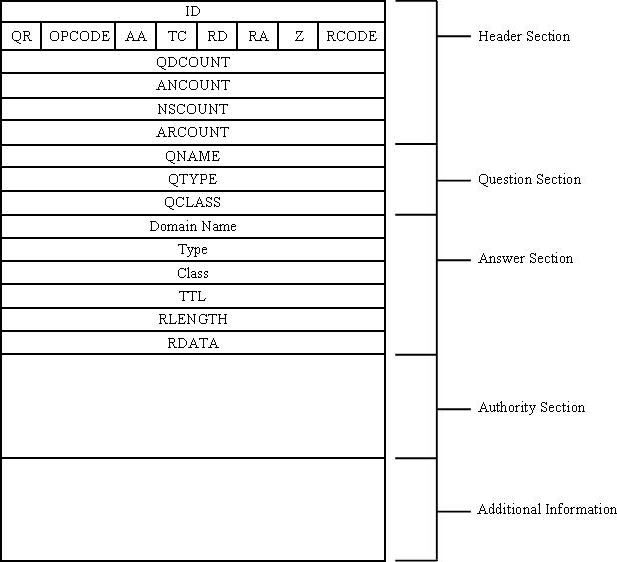
\includegraphics[scale=1]{inc/img/DNS.png}}
		\caption{Общая структура DNS-пакета.}
		\label{img:DNS}
	\end{center}
\end{figure} 

\subsection{Поле заголовка}

В поле заголовка содержится информация о пакете, его назначении и количестве данных, содержащихся в каждом поле данных.

\begin{itemize}
	\item Биты 0-15: ID -- уникальный 16-битовый идентификационный номер пакета запроса. Пакет ответа, формируемый сервером, также использует этот идентификационный номер, чтобы клиент мог сопоставить ответ сервера со своим запросом.
	\item Бит 16: QR -- тип пакета (0 -- пакет запроса, 1 -- пакет ответа). 
	\item Биты 17-20: OPCODE -- тип запроса: стандартный (0), обратный (1) или запрос о статусе сервера (2) (номера 3-15 зарезервированы на будущее).
	\item Бит 21: AA -- устанавливается, когда ответ является авторитетным (то есть данные поступают напрямую от DNS-сервера, ответственного за зону). Неавторитетные ответы могут поступать от серверов DNS, в кэше которых сохранилась информация об исходных записях от предыдущих запросов.
	\item Бит 22: TC -- устанавливается, если сервер не смог поместить всю необходимую информацию в пакет из-за существующих ограничений.
	\item Бит 23: RD -- устанавливается в запросе и копируется в ответ, если клиент просит сервер не сообщать ему промежуточных ответов, а вернуть только IP-адрес.
	\item Бит 24: RA -- устанавливается, чтобы уведомить клиента о возможности рекурсивного запроса на данный сервер.
	\item Биты 25-27: Z -- в настоящее время не используются и зарезервированы на будущее.
	\item Биты 28-31: RCODE -- используются только в пакетах ответов и отображают состояние ответа: 
	\begin{itemize}
		\item 0 -- без ошибок;
		\item 1 -- ошибки в пакете запроса;
		\item 2 -- внутренние ошибки не дали возможности серверу обработать запрос;
		\item 3 -- имя, указанное в запросе, не существует;
		\item 4 -- данный тип запроса не поддерживается сервером;
		\item 5 --  сервер не может удовлетворить запрос клиента в силу административных ограничений безопасности.
	\end{itemize}
\end{itemize}

Остальные четыре параметра заголовка представляют собой 16-битные числа и используются для учета количества исходных записей, возвращаемых в пакете:
\begin{itemize}
	\item Биты 28-31: QDCOUNT -- количество записей в поле запросов;
	\item Биты 28-31: ANCOUNT — количество записей в поле ответов;
	\item Биты 28-31: NSCOUNT -- количество записей в поле об авторитетных серверах имен;
	\item Биты 28-31: ARCOUNT -- количество записей в поле дополнительной информации.
\end{itemize}

 
\subsection{Поле запроса}
Поле запроса содержит запросы, ответы на которые клиент желает получить от DNS-сервера, и состоит из трех частей.

\begin{enumerate}
	\item QNAME -- список имен, для которых клиент желает получить IP-адреса. Перед каждым именем ставится однобайтное значение, которое определяет длину имени, а конец списка обозначается именем с нулевой длиной.
	\item QTYPE -- в каком виде клиент желает принимать информацию об имеющихся доменах (МХ, A, TXT и т.д.).
	\item QCLASS -- класс запроса (для сети Internet -- IN).
\end{enumerate}


\subsection{Поля ответа, полномочий и дополнительной информации}

В поле ответа содержатся исходные записи базы DNS, доступные на сервере на момент запроса клиента. Если бит заголовка АА не установлен, то в поле полномочий будут указаны DNS-серверы, к которым клиент может обращаться за авторитетными ответами. В поле дополнительной информации передаются все исходные записи, которые воспринимаются DNS-сервером как имеющие отношение к данному запросу.

Поля ответа, полномочий и дополнительной информации имеют одинаковый формат:
\begin{itemize}
	\item NAME -- доменное имя, относящееся к исходной записи (тот же формат, что и QNAME в секции запроса);
	\item TYPE -- тип исходной записи;
	\item CLASS	-- класс исходной записи (IN для Internet);
	\item TTL -- допустимое время хранения данной ресурсной записи 
	в кэше неавторитетного DNS-сервера;
	\item RDLENGTH -- длина поля данных в записи;
	\item RDATA	-- поле данных (формат зависит от типа записи).
\end{itemize}



\section{Правила фильтрации}

Для фильтрации сетевых пакетов принято учитывать следующие параметры:
\begin{itemize}
	\item протокол передачи;
	\item ip-адрес источника;
	\item ip-адрес назначения;
	\item порт источника;
	\item порт назначения.
\end{itemize}

Особенности работы протоколов передачи пакетов в данной работе не рассматриваются.

Перечисленных выше параметров зачастую оказывается недостаточно. Например, когда на хост осуществляется спуфинг-атака (от англ. spoofing -- подмена).

% пытается осуществить кибер-атаку, называемую IP-Spoofing (Спуфинг с подменой IP-адреса)\cite{spoof}. 

Спуфинг -- это кибер-атака, в рамках которой мошенник выдает себя за некоторый надежный источник, чтобы получить доступ к важным данным или информации\cite{spoof}. Различают несколько видов спуфинг-атак, в данной работе будут рассмотрены два из них.

\begin{enumerate}
	\item IP-спуфинг. Данный вид спуфинга заключается в замене реальных ip-адресов на поддельные. Это дает возможность скрывать местоположение мошенника в интернете, перенаправлять данные пользователя к ненадежным устройствам и т\,д.. Защитой от простейших попыток таких атак является использование двух правил~\cite{blockspoof}.
	\begin{enumerate}
		\item Отклонять любой входящий пакет с ip-адресом сети защищаемого хоста в качестве ip-адреса источника для любых номеров портов и протоколов. Логика этого правила в том, что на межсетевой экран не может  прийти пакет в сеть защищаемого хоста, и при этом в нем указано, что послан он из этой же сети. %Это означает, что кто-то его подделал и пытается замаскироваться под одного из пользователей.
		\item Не выпускать пакет из внутренней сети, если в нем указан ip-адрес источника, отличный от внутренних адресов сети (логика данного правила аналогична).
	\end{enumerate}

	\item DNS-спуфинг. В данном виде спуфинга DNS-кэш хоста или некоторого промежуточного DNS-сервера заполняется поддельными данными, в результате чего пользователь получает некорректный ip-адрес и  перенаправляется на вредоносный сайт. Один из способов защиты от DNS-спуфинг -- запрет на получение ответов от неавторитетных серверов, так как их кэш может быть <<отравлен>>. Для этого необходимо проверять бит AA поля заголовка DNS-пакета.
\end{enumerate}

%Когда мошенник стремится скрыть реальное местоположение в Интернете того места, откуда запрашиваются или куда отправляются данные пользователя, обычно используется спуфинг с подменой IP-адреса. Цель IP-спуфинга состоит в том, чтобы заставить компьютер жертвы думать, что обмен информацией происходит с надежным источником.



\section{Выводы}

В результате проведенного анализа был определен способ перехвата входящих и исходящих пакетов -- путем регистрации функций перехвата с использованием библиотеки Netfilter. В качетсве точек перехвата предлагается использовать точку, которую проходят все входящие пакеты \\(NF\_INET\_PRE\_ROUTING), и точку, которую проходят все исходящие пакеты (NF\_INET\_POST\_ROUTING).

Были рассмотрены структуры и функции ядра, предоставляющие  информацию о сетевых пакетах, а также структура DNS-пакетов. Определены параметры правил фильтрации и способы защиты от спуфинг-атак.
